%	This is written by Zhiyang Ong as a template for writing reports.

%	The MIT License (MIT)

%	Copyright (c) <2014> <Zhiyang Ong>

%	Permission is hereby granted, free of charge, to any person obtaining a copy of this software and associated documentation files (the "Software"), to deal in the Software without restriction, including without limitation the rights to use, copy, modify, merge, publish, distribute, sublicense, and/or sell copies of the Software, and to permit persons to whom the Software is furnished to do so, subject to the following conditions:

%	The above copyright notice and this permission notice shall be included in all copies or substantial portions of the Software.

%	THE SOFTWARE IS PROVIDED "AS IS", WITHOUT WARRANTY OF ANY KIND, EXPRESS OR IMPLIED, INCLUDING BUT NOT LIMITED TO THE WARRANTIES OF MERCHANTABILITY, FITNESS FOR A PARTICULAR PURPOSE AND NONINFRINGEMENT. IN NO EVENT SHALL THE AUTHORS OR COPYRIGHT HOLDERS BE LIABLE FOR ANY CLAIM, DAMAGES OR OTHER LIABILITY, WHETHER IN AN ACTION OF CONTRACT, TORT OR OTHERWISE, ARISING FROM, OUT OF OR IN CONNECTION WITH THE SOFTWARE OR THE USE OR OTHER DEALINGS IN THE SOFTWARE.

%	Email address: echo "cukj -wb- 23wU4X5M589 TROJANS cqkH wiuz2y 0f Mw Stanford" | awk '{ sub("23wU4X5M589","F.d_c_b. ") sub("Stanford","d0mA1n"); print $5, $2, $8; print " "; for (i=1; i<=1; i++) print "6\b"; print $9, $7, $6 }' | sed y/kqcbuHwM62z/gnotrzadqmC/ | tr 'q' ' ' | tr -d "\n" | tr -d 'ir' | tr y "\n"

%%%%%%%%%%%%%%%%%%%%%%%%%%%%%%%%%%%%%%%%%%%%%%









%%%%%%%%%%%%%%%%%%%%%%%%%%%%%%%%%%%%%%%%%%%%%%
%	Preamble.
\documentclass[letterpaper,12pt]{report}
%%%%%%%%%%%%%%%%%%%%%%%%%%%%%%%%%%%%%%%%%%%%%
%
%	Importing LaTeX source files, without quoting the ".tex" extension.
%
%%%%%%%%%%%%%%%%%%%%%%%%%%%%%%%%%%%%%%%%%%%%%

%%%%%%%%%%%%%%%%%%%%%%%%%%%%%%%%%%%%%%%%%%%%%
%	File containing the LaTeX preamble.
% This is written by Zhiyang Ong as the preamble for all his LaTeX documents.
%
% It includes a list of LaTeX packages that he commonly uses to typeset LaTeX documents.

%	The MIT License (MIT)

%	Copyright (c) <2014> <Zhiyang Ong>

%	Permission is hereby granted, free of charge, to any person obtaining a copy of this software and associated documentation files (the "Software"), to deal in the Software without restriction, including without limitation the rights to use, copy, modify, merge, publish, distribute, sublicense, and/or sell copies of the Software, and to permit persons to whom the Software is furnished to do so, subject to the following conditions:

%	The above copyright notice and this permission notice shall be included in all copies or substantial portions of the Software.

%	THE SOFTWARE IS PROVIDED "AS IS", WITHOUT WARRANTY OF ANY KIND, EXPRESS OR IMPLIED, INCLUDING BUT NOT LIMITED TO THE WARRANTIES OF MERCHANTABILITY, FITNESS FOR A PARTICULAR PURPOSE AND NONINFRINGEMENT. IN NO EVENT SHALL THE AUTHORS OR COPYRIGHT HOLDERS BE LIABLE FOR ANY CLAIM, DAMAGES OR OTHER LIABILITY, WHETHER IN AN ACTION OF CONTRACT, TORT OR OTHERWISE, ARISING FROM, OUT OF OR IN CONNECTION WITH THE SOFTWARE OR THE USE OR OTHER DEALINGS IN THE SOFTWARE.

%	Email address: echo "cukj -wb- 23wU4X5M589 TROJANS cqkH wiuz2y 0f Mw Stanford" | awk '{ sub("23wU4X5M589","F.d_c_b. ") sub("Stanford","d0mA1n"); print $5, $2, $8; for (i=1; i<=1; i++) print "6\b"; print $9, $7, $6 }' | sed y/kqcbuHwM62z/gnotrzadqmC/ | tr 'q' ' ' | tr -d [:cntrl:] | tr -d 'ir' | tr y "\n"

%%%%%%%%%%%%%%%%%%%%%%%%%%%%%%%%%%%%%%%%%%%%%%%%%%

% Importing some standard LaTeX packages.

% To enable standard LaTeX processing for graphics. It enables PDF, JPEG, PNG, and TIFF graphics files to be included in the LaTeX document.
\usepackage{graphicx}
% For better typesetting of mathematical expressions, from the American Mathematical Society (AMS).
\usepackage{amsmath}
% For better typesetting of mathematical expressions, from the American Mathematical Society (AMS). This package includes mathematical symbols for the ``amsmath'' package.
\usepackage{amssymb}
% For better typesetting of mathematical proofs (for theorems and colloraries), from the American Mathematical Society (AMS).
\usepackage{amsthm}
%	Create definitions for new theorems, axioms, colloraries.
	\newtheorem{theorem}{Theorem}[chapter]
	\newtheorem{axiom}{Axiom}[chapter]
	\newtheorem{corollary}{Corollary}[chapter]
	\newtheorem{lemma}{Lemma}[chapter]
	\newtheorem{Rule}{Rule}[chapter]
	\newtheorem{law}{Law}[chapter]
	\newtheorem{principle}{Principle}[chapter]
% To change the style of newly defined theorems.
%		\usepackage{theorem}
%	Enable the use of right-sided cases.
\usepackage{mathtools}



%	Typesetting with the typewriter font.
%\usepackage{ttfamily}

% For better typesetting of tables (and arrays).
\usepackage{array}
% For creating tables without vertical separators.
%		\usepackage{booktabs}
% To control line spacing in LaTeX documents.
\usepackage{setspace}
% To modify the spacing between words and letters.
%		\usepackage{microtype}
% To change the dimensions of the page(s).
%\usepackage[margin=1.5cm,vmargin={0pt,1cm},nohead]{geometry}
\usepackage[margin=1.5cm,vmargin={1.5cm,2cm}]{geometry}
% Use the packages needed to typeset algorithms. I can also use the combined ``algorithms'' bundle.
\usepackage{algorithm}
\usepackage{algorithmic}
% The listings package is a source code printer for LaTeX. You can typeset stand alone files as well as listings with an environment similar to verbatim as well as you can print code snippets using a command similar to \verb. Many parameters control the output and if your preferred programming language isn't already supported, you can make your own definition.
\usepackage{listings}
% Use the ``clrscode3e'' LaTeX package to typeset algorithms like CLRS
%	\usepackage{/data/others/notes/clrscode3e}
%/Applications/apps/comune/SienaLaTeX/rapporto/
%\usepackage{/Applications/apps/comune/SienaLaTeX/rapporto/others/clrscode3e}
\usepackage{others/packages/clrscode3e}
%\usepackage{/data/others/grappanotes/clrscode3e}
% Use the ``algpseudocode'' LaTeX package to typeset algorithms -- Alternate solution, not preferred
%\usepackage{algpseudocode}
% Alternative packages for typesetting algorithms.
%\usepackage{algorithm2e}
%\usepackage{algorithmicx}
%\usepackage{program}
%	To check for syntax errors in my LaTeX document.
\RequirePackage[l2tabu, orthodox]{nag}

% Concatenate adjacent references together when typeset.
% That is, cite{ref1,ref2,ref3,ref4} can appear as [12-15], instead of [12] [13] [14] [15]
\usepackage{cite}
% For automatic insertion of cross-referencing words, such as fig. for figures and eq. for equations.
%		\usepackage{cleveref}

% LaTeX support for Metafont and MetaPost logos.
\usepackage{mflogo}













% How to typeset single and double quotes for feet and inches?
% For feet, use [FEET]\textasciiacute
% For inches, use [INCHES]\textacutedbl
% For feet and inches, use [FEET]\textasciiacute\ [INCHES]\textacutedbl; force a character space between the single quote for feet and the height of the object in inches
% Don't use \textceltpal as a single quote to represent height in feet, or double \textceltpal (two concatenated \textceltpal) as a double quote to represent height in inches
% For double quotes, don't use two single quotes provided by the default settings of LaTeX. The resultant double quotes will be curly.

% The tipa package is for Phonetic Symbols -- I wanna use the \textceltpal symbol to represent a single quote, instead of using the generic ``curly'' single quote from \LaTeX (Table 10, pp.10)
\usepackage{tipa}
% The textcomp package is for Diacritics -- I wanna use the \textacutedbl symbol to represent a double quote (Table 28, pp.17), instead of using the generic ``curly'' double quotes from \LaTeX; however, when this symbol is used, I must force a character space to exist after the symbol by using the backslash followed by a character space. This package also provides the symbol for Copyleft, \textcopyleft, which is not available in LaTeX by default, and provides better looking symbols for: copyright, registered, and trademark (Table 33, pp.18). Also, it provides symbols for: \textcelsius, \textmho, \textmu, \textohm (Table 201, pp.67). It also provides symbols for Genealogical Symbols (Table 253, pp78), such as \textborn, \textdivorced, \textmarried, \textdied, and \textleaf (symbol of a leaf)... Its symbol for the Euro, EU currency, is \texteuro
\usepackage{textcomp}
% Look at \url{http://www.ctan.org/tex-archive/info/symbols/comprehensive/symbols-a4.pdf} for a list of symbols that can be used in LaTeX and its packages. Table 280, pp.88, deals with Symbol Name Clashes; hence, if the same command name refers to multiple symbols, the symbol-conflict resolution abides by this.
% In particular, check out the gensymb package (Table 197, page 67) for symbols defined to work in both math and text modes, such as \celsius, \micro, \degree, and \ohm.
% Also, check out the wasysym package (Table 198, page 67) for electrical symbols, such as that of alternating current (AC); it also provides symbols for \female, and \male (Table 212, pp.70); it also has symbols for ``Xs and Check Marks,'' which are checked boxes, \CheckedBox, squares, \Square, and crossed boxes (boxes filled with a cross), \XBox (Table 232, pp.73); it also has symbols for a clock, \clock, a Simley, \smiley, diameter, \diameter, lightning, \lightning, sun, \sun, and a tick or check mark \checked (symbol to indicate that something is correct), and a bell, \bell (Table 254, pp.78); it also has symbols for left and right turns (Table 256, pp.78), \leftturn and \rightturn; this package (Table 256, pp.78) and the arev package (Table 257, pp.78) can be used to typeset music symbols, along with Table 182, pp.62; it also has symbols for Navigation (Table 261, pp.79), such as \Forward, \RewindToStart, and \ForwardToIndex; it also has symbols for laundry (Table 262, pp.80); it also has the symbol for a heart, \Heart (Table 263, pp.80).
% In addition, check out the ifsym package (Table 199, page 67) for pulse diagram symbols; it also has symbols for weather (Table 266, pp.80), alpine and mountain climbing, such as \Summit, \Mountain, \IceMountain, \VarMountain, \Flag, \FilledHut, \Hut, \Village, and \Tent (Table 267, pp.81); it also has different symbols for clocks, such as \Interval, \StopWatchEnd, \VarClock, \showclock (to indicate the time) (Table 268, pp.81); it also has symbols for fire, letter, telephone, dice, \PaperPortrait, and \PaperLandscape. Also, has symbol for the cross to indicate that something is incorrect
\usepackage{ifsym}
% Besides, check out the keystroke package (Table 208, page 69) for symbols of Computer Keys, such as Alt, Ctrl, Del, Page down, Esc, Enter, Shift, Space Bar, and Up Arrow.
% From the dingbat package (Table 225, page 72), it has symbols for Fists, such as \rightthumbsdown and \rightthumbsup.
%\usepackage{dingbat}
% From the pifont package (Table 234, page 73), it has symbols for Circled Numbers, such as any digit that is circled, where the space in the circle can be shaded black.
% From the dictsym package (Table 277, page 84), it has symbols for dictionaries, and indicates which type of dictionary will define this term - say a medical, technical, mathematical, or judical dictionary
% The simpsons package can be used to indicate characters from {\it The Simpsons} (Table 278, pp.85)
% The symbol for quadruple integrals \iiiint is available as an AMS Variable-sized Math Operator, or I can use this symbol from the packages txfonts, pxfonts, esint, or MnSymbol 










% The marvosym package (Table 210, page 69) is for Communication Symbols, such as \Email, \fax, \FAX (Preferred), \Letter, \Mobilefone, and \Telefon; it also has the symbol for the Cross to represent Christianity, \Cross (Table 263, pp.80); it also has symbols for checked boxes, \Checkedbox, crossed boxes (boxes marked with a cross), \Crossedbox, bicycles, \Bicycle, clocks, \Clocklogo, the industry, \Industry, taking notes manually with pen/pencil and paper, \Writinghand, coffee, \Coffeecup, providing information or important note, \Info (Table 249, pp.76)... In addition, it has the symbols for the Euro (EU currency), \EUR (OK), \EURdig (OK), \EURtm, \EURcr
\usepackage{marvosym}
% From the bbding package (Table 226, page 72), it has symbols for Fists, such as \HandPencilLeft; it also has symbols for the Cross to represent Christianity, such as \Cross and \CrossOpenShadow (Table 228, pp.72); Use of the symbol \Cross has bugs; bugs exist in the package, as it fails to correctly overwrite the \Cross symbol; also has the peace symbol, \Peace. 
%\usepackage{bbding}
% The skak contains a cross, incorrect symbol that I can use to indicate that something is wrong, e.g. \markera or \weakpt
\usepackage{skak}
% Package to enable the use of a strikeout/strikethrough font with LaTeX. To use the strikeout/strikethrough font, use the ``sout'' LaTeX command, or tag,  to ``strike through'' text. E.g., \sout{Bill Clinton} G.W. Bush is the pres.
\usepackage{ulem}
% The eurosym package has the symbols for the Euro (EU currency), \geneuro, \geneuronarrow, \geneurowide, \officialeuro (GOOD)
\usepackage{eurosym}











% Create fancy headers and footers for this document
\usepackage{fancyhdr}
\setlength{\headheight}{15.2pt}
\pagestyle{fancy}
% Headers for the document
\lhead{}
%\lhead{Zhiyang Ong}
%\rhead{\today}
% Footers for the document
\lfoot{Zhiyang Ong}
\cfoot{}
\rfoot{\thepage}

% The following does not work, since it does not differentiate between odd and even pages. Hence, the last odd/even command will overwrite the previous even/odd command
%\fancyhf{}
%\fancyhead[LE]{Author's DFM}
%\fancyhead[LO]{\today EDA}
%\fancyfoot[LE]{\thepage USC}
%\fancyfoot[RO]{\thepage Adel}


% Allow for multi-line comments
\usepackage{verbatim}




% Commands for using the package for hyperlinks. Includes the package ``url''.
\usepackage[pdftex,
	pdftitle={Graphics and Color with LaTeX},
	pdfauthor={Patrick W Daly},
	pdfsubject={Importing images and use of color in LaTeX},
	pdfkeywords={LaTeX, graphics, color},
	pdfpagemode=UseOutlines,bookmarks, bookmarksopen,
	pdfstartview=FitH, colorlinks, linkcolor=blue, citecolor=blue, urlcolor=red,
]{hyperref}
\hypersetup{colorlinks, linkcolor=blue}







% Create a glossary for symbols and terms in this document
% The following attempt failed
%\makeglossaries

% The following attempt failed
%%%%%%%%%%%%%%%%%%%%%%%%%%%%%\makeglossary
%\usepackage{supertabular}
%\newcommand{\glossaryname}{Symbols Index}
%\newenvironment{theglossary}
%    {\section*{Symbols Index}
%      \begin{supertabular}{ll}}
%    {\end{supertabular}
%}
%\newcommand{\printglossary}{\InputIfFileExists{zhiyang_ong.glo}{}{\section*{Symbols Index - File not found}}}

% Another failed attempt at creating a glossary
%\input{gatech-thesis-gloss.sty}
%\usepackage{gatech-thesis-gloss}
%\glossfiles{zhiyang_ong.glo}

% Create the glossary
\usepackage{nomencl}
\makenomenclature


% Enable captions to be modified.
%\usepackage{caption}
% Addition support for colored text.
%\usepackage{color}
% Enable the insertion of PDF/PS files/documents.
		\usepackage{pdfpages}
% To rotate objects, including tables.
		\usepackage{rotating}
% To define multiple floats (figures and tables), with individual captions and labels, within one environment.
		\usepackage{subfig}
% For a modular LaTeX document with multiple files (including the ``root file''), it allows the a non-empty subset of the ``child files'' to be typeset without having to typeset the ``root file'' (and/or the other ``child files'').
		\usepackage{subfiles}
% To annotate the LaTeX document with to-do notes.
		\usepackage[colorinlistoftodos]{todonotes}
% To insert images surrounded by text.
		\usepackage{wrapfig}
% To create trees, graphs, (commutative) diagrams, and similar things. Reference: Wikibooks contributors, ``\LaTeX/Xy-pic,'' in {\it \LaTeX}, Wikibooks: Open books for an open world, Wikimedia Foundation, San Francisco, CA, June 5, 2005. Available online at: \url{http://en.wikibooks.org/wiki/LaTeX/Xy-pic}; last accessed on December 25, 2013.		=> This package seems to have bugs in it. If I use this package, my document will not typeset properly. I have tried to use it successfully in other documents. It does not seem to be compatible with 
%\usepackage{xypic}
% Package for SI units.
\usepackage{siunitx}






%	For typesetting the symbol: \AE.
\usepackage[T1]{fontenc}
\usepackage[utf8]{inputenc}
\usepackage{lmodern}





%	Allow modification of how enumeration is done.
\usepackage{enumitem}







%%%%%%%%%%%%%%%%%%%%%%%%%%%%%%%%%%%%%%%%%%%%%%%%%%
% Other helpful hints:

% To use the italic and bold font concurrently, try this: {\itshape Review the {\bfseries updated} training log}

% To use the symbol for summation, which is the capital-sigma notation, with proper super- and sub- fixes, try: $\displaystyle\sum_{i = -1}^{m} \frac{log_2 n_i}{T_i}$

% Make sure that I include the following so that I can cite references properly: \usepackage{cite}. This allows references to be included as [1-10], rather than [1], [2], [3], [4], [5], [6], [7], [8], [9], [10]

% Colors that appear well in PDF format for LaTeX text include: red, blue, and magenta

% Use \scriptsize, instead of \textsc, \sc, or \schape to use small caps. Currently, I cannot use \textsc, \sc, or \schape to write in small caps on my MacBook Pro laptop.

% The Typewriter font cannot be used concurrently with the bold font. That is, the following cannot be used: {\tt \bf text}, AND \texttt{\textbf{text}}

% Use \LaTeX for LaTeX; B{\scriptsize IB}\TeX to indicate the symbol for BibTeX; \texttrademark for trademarks; \MF for Metafont; and \MP for MetaPost




%%%%%%%%%%%%%%%%%%%%%%%%%%%%%%%%%%%%%%%%%%
%																%
%	Default colors that I can use with \LaTeX:								%
%	1) red														%
%	2) green														%
%	3) blue														%
%	4) yellow														%
%	5) cyan														%
%	6) magenta													%
%	7) black														%
%	8) white														%
%																%
%%%%%%%%%%%%%%%%%%%%%%%%%%%%%%%%%%%%%%%%%%


% Partial list of ``the 68 predefined internal colors of the {\tt dvips} PostScript driver'' \cite{Kopka04} that I can use for changing the color of text ... Use bold font for the text
%YellowOrange
%RoyalBlue
%DarkOrchid
%ForestGreen
%OliveGreen
%Mulberry
%ProcessBlue
%RubineRed
%VioletRed
%WildStrawberry
% E.g., try: \textcolor{VioletRed}{\bf hello world}

% As for changing the background color of text, choose a light colored background to make the text stand out in black colored bold font; see \url{oregonstate.edu/~peterseb/tex/samples/docs/color-package-demo.pdf} for a list of colors
% E.g., try: \colorbox{Apricot}{\bf hello world}
%	Enable the use of right-sided cases.
\usepackage{mathtools}
%\usepackage{extarrows}
\usepackage{combelow}





%%%%%%%%%%%%%%%%%%%%%%%%%%%%%%%%%%%%%%%%%%%%%
%
%	Start of LaTeX document
%
%%%%%%%%%%%%%%%%%%%%%%%%%%%%%%%%%%%%%%%%%%%%%
\begin{document}

%%%%%%%%%%%%%%%%%%%%%%%%%%%%%%%%%%%%%%%%%
%	File containing a list of ``the 68 predefined internal colors of the {\tt dvips} PostScript driver'' \cite{Kopka04} 
%	This allows me to use any of these ``68 predefined internal colors''
% This is written by Zhiyang Ong to recreate the ``68 predefined internal colors of the {\tt dvips} PostScript driver'' \cite{Kopka04}
%
%
% I have written this because I cannot get the aforementioned 68 predefined internal colors to work for any \LaTeX document on my MacBook Pro. Perhaps the \LaTeX\ setup is the cause of the problem.
% I have used the \usepackage{color} command with the ``dvipsnames'' and ``usenames'' options to no avail
% The \usepackage{color} command with the aforementioned options are added into the preamble \cite{Kopka04} and see \url{http://oregonstate.edu/~peterseb/tex/samples/color-package.html} (last viewed Monday, May 25, 2009 @ 0900 hrs PST)
% \usepackage[dvipsnames]{color}
% \usepackage[usenames]{color}
%
%
% Hence, I used a file ``dvipsnam.def'' containing the list of these 68 predefined internal colors to create the definitions of these 68 colors for use in my \LaTeX\ document(s)
% The original source file is located at \url{http://spib.ece.rice.edu/E-Pub/color/dvipsnam.def}
% This source file is provided in the Signal Processing Information Base (SPIB), which is made available by courtesy of the Department of Electrical and Computer Engineering, Rice University
%
%	The MIT License (MIT)
%
%	Copyright (c) <2014> <Zhiyang Ong>
%
%	Permission is hereby granted, free of charge, to any person obtaining a copy of this software and associated documentation files (the "Software"), to deal in the Software without restriction, including without limitation the rights to use, copy, modify, merge, publish, distribute, sublicense, and/or sell copies of the Software, and to permit persons to whom the Software is furnished to do so, subject to the following conditions:
%
%	The above copyright notice and this permission notice shall be included in all copies or substantial portions of the Software.
%
%	THE SOFTWARE IS PROVIDED "AS IS", WITHOUT WARRANTY OF ANY KIND, EXPRESS OR IMPLIED, INCLUDING BUT NOT LIMITED TO THE WARRANTIES OF MERCHANTABILITY, FITNESS FOR A PARTICULAR PURPOSE AND NONINFRINGEMENT. IN NO EVENT SHALL THE AUTHORS OR COPYRIGHT HOLDERS BE LIABLE FOR ANY CLAIM, DAMAGES OR OTHER LIABILITY, WHETHER IN AN ACTION OF CONTRACT, TORT OR OTHERWISE, ARISING FROM, OUT OF OR IN CONNECTION WITH THE SOFTWARE OR THE USE OR OTHER DEALINGS IN THE SOFTWARE.
%
%	Email address: echo "cukj -wb- 23wU4X5M589 TROJANS cqkH wiuz2y 0f Mw Stanford" | awk '{ sub("23wU4X5M589","F.d_c_b. ") sub("Stanford","d0mA1n"); print $5, $2, $8; for (i=1; i<=1; i++) print "6\b"; print $9, $7, $6 }' | sed y/kqcbuHwM62z/gnotrzadqmC/ | tr 'q' ' ' | tr -d [:cntrl:] | tr -d 'ir' | tr y "\n"

%%%%%%%%%%%%%%%%%%%%%%%%%%%%%%%%%%%%%%%%%%%%%%



%%%%%%%%%%%%%%%%%%%%%%%%%%%%%%%%%%%%%%%
% Text retained from the header of the original ``dvipsnam.def'' file
%%
%% This is file `dvipsnam.def',
%% generated with the docstrip utility.
%%
%% The original source files were:
%%
%% drivers.dtx  (with options: `dvipsnames')
%% 
%% drivers.dtx Copyright (C) 1994      David Carlisle Sebastian Rahtz
%%             Copyright (C) 1995 1996 1997 1998 1999 David Carlisle
%%
%% This file is part of the Standard LaTeX `Graphics Bundle'.
%% It may be distributed under the terms of the LaTeX Project Public
%% License, as described in lppl.txt in the base LaTeX distribution.
%% Either version 1.0 or, at your option, any later version.
%%




%%%%%%%%%%%%%%%%%%%%%%%%%%%%%%%%%%%%%%%
% Commence definition of ``the 68 predefined internal colors of the {\tt dvips} PostScript driver'' \cite{Kopka04}
\definecolor{GreenYellow}{cmyk}{0.15,0,0.69,0}
\definecolor{Yellow}{cmyk}{0,0,1,0}
\definecolor{Goldenrod}{cmyk}{0,0.10,0.84,0}
\definecolor{Dandelion}{cmyk}{0,0.29,0.84,0}
\definecolor{Apricot}{cmyk}{0,0.32,0.52,0}
\definecolor{Peach}{cmyk}{0,0.50,0.70,0}
\definecolor{Melon}{cmyk}{0,0.46,0.50,0}
\definecolor{YellowOrange}{cmyk}{0,0.42,1,0}
\definecolor{Orange}{cmyk}{0,0.61,0.87,0}
\definecolor{BurntOrange}{cmyk}{0,0.51,1,0}
\definecolor{Bittersweet}{cmyk}{0,0.75,1,0.24}
\definecolor{RedOrange}{cmyk}{0,0.77,0.87,0}
\definecolor{Mahogany}{cmyk}{0,0.85,0.87,0.35}
\definecolor{Maroon}{cmyk}{0,0.87,0.68,0.32}
\definecolor{BrickRed}{cmyk}{0,0.89,0.94,0.28}
\definecolor{Red}{cmyk}{0,1,1,0}
\definecolor{OrangeRed}{cmyk}{0,1,0.50,0}
\definecolor{RubineRed}{cmyk}{0,1,0.13,0}
\definecolor{WildStrawberry}{cmyk}{0,0.96,0.39,0}
\definecolor{Salmon}{cmyk}{0,0.53,0.38,0}
\definecolor{CarnationPink}{cmyk}{0,0.63,0,0}
\definecolor{Magenta}{cmyk}{0,1,0,0}
\definecolor{VioletRed}{cmyk}{0,0.81,0,0}
\definecolor{Rhodamine}{cmyk}{0,0.82,0,0}
\definecolor{Mulberry}{cmyk}{0.34,0.90,0,0.02}
\definecolor{RedViolet}{cmyk}{0.07,0.90,0,0.34}
\definecolor{Fuchsia}{cmyk}{0.47,0.91,0,0.08}
\definecolor{Lavender}{cmyk}{0,0.48,0,0}
\definecolor{Thistle}{cmyk}{0.12,0.59,0,0}
\definecolor{Orchid}{cmyk}{0.32,0.64,0,0}
\definecolor{DarkOrchid}{cmyk}{0.40,0.80,0.20,0}
\definecolor{Purple}{cmyk}{0.45,0.86,0,0}
\definecolor{Plum}{cmyk}{0.50,1,0,0}
\definecolor{Violet}{cmyk}{0.79,0.88,0,0}
\definecolor{RoyalPurple}{cmyk}{0.75,0.90,0,0}
\definecolor{BlueViolet}{cmyk}{0.86,0.91,0,0.04}
\definecolor{Periwinkle}{cmyk}{0.57,0.55,0,0}
\definecolor{CadetBlue}{cmyk}{0.62,0.57,0.23,0}
\definecolor{CornflowerBlue}{cmyk}{0.65,0.13,0,0}
\definecolor{MidnightBlue}{cmyk}{0.98,0.13,0,0.43}
\definecolor{NavyBlue}{cmyk}{0.94,0.54,0,0}
\definecolor{RoyalBlue}{cmyk}{1,0.50,0,0}
\definecolor{Blue}{cmyk}{1,1,0,0}
\definecolor{Cerulean}{cmyk}{0.94,0.11,0,0}
\definecolor{Cyan}{cmyk}{1,0,0,0}
\definecolor{ProcessBlue}{cmyk}{0.96,0,0,0}
\definecolor{SkyBlue}{cmyk}{0.62,0,0.12,0}
\definecolor{Turquoise}{cmyk}{0.85,0,0.20,0}
\definecolor{TealBlue}{cmyk}{0.86,0,0.34,0.02}
\definecolor{Aquamarine}{cmyk}{0.82,0,0.30,0}
\definecolor{BlueGreen}{cmyk}{0.85,0,0.33,0}
\definecolor{Emerald}{cmyk}{1,0,0.50,0}
\definecolor{JungleGreen}{cmyk}{0.99,0,0.52,0}
\definecolor{SeaGreen}{cmyk}{0.69,0,0.50,0}
\definecolor{Green}{cmyk}{1,0,1,0}
\definecolor{ForestGreen}{cmyk}{0.91,0,0.88,0.12}
\definecolor{PineGreen}{cmyk}{0.92,0,0.59,0.25}
\definecolor{LimeGreen}{cmyk}{0.50,0,1,0}
\definecolor{YellowGreen}{cmyk}{0.44,0,0.74,0}
\definecolor{SpringGreen}{cmyk}{0.26,0,0.76,0}
\definecolor{OliveGreen}{cmyk}{0.64,0,0.95,0.40}
\definecolor{RawSienna}{cmyk}{0,0.72,1,0.45}
\definecolor{Sepia}{cmyk}{0,0.83,1,0.70}
\definecolor{Brown}{cmyk}{0,0.81,1,0.60}
\definecolor{Tan}{cmyk}{0.14,0.42,0.56,0}
\definecolor{Gray}{cmyk}{0,0,0,0.50}
\definecolor{Black}{cmyk}{0,0,0,1}
\definecolor{White}{cmyk}{0,0,0,0}









%%%%%%%%%%%%%%%%%%%%%%%%%%%%%%%%%%%%%%%%%%%%%
%%%%%%%%%%%%%%%%%%%%%%%%%%%%%%%%%%%%%%%%%%%%%
%
%	Information for Top Matter / Title page
%
%%%%%%%%%%%%%%%%%%%%%%%%%%%%%%%%%%%%%%%%%%%%%
%%%%%%%%%%%%%%%%%%%%%%%%%%%%%%%%%%%%%%%%%%%%%
%	Beginning of FRONT MATTER: title page, table of contents and prefaces
%	Note that the \vspace{length} command does NOT work for the front matter
%\frontmatter
\title{\Huge \bf Title of the Report: Some Details about the Report}

%	Indicate the date of the report.
\date{\today}

\author{{\LARGE Name Surname}
\thanks{Email correspondence to: \href{mailto:email-id@domain.url}{\Email\ email-id@domain.url}}
\ \\
\vspace{-4.0in}
\ \\
\ \\
\ \\
{\bf \LARGE
	Name of Organization
	\vspace{0.1cm}} \\
\hline
\ \\
{\Large \sc Name of Group/Division} \\
\ \\
\ \\
\ \\
\ \\
\ \\
\vspace{2.0in}
\ \\
{\large \sc What is this report for?} \\
{\large It is for \dots} \\
{\large and BLAH \dots}
}

%	Create the title page.
\maketitle


%%%%%%%%%%%%%%%%%%%%%%%%%%%%%%%%%%%%%%%%%%%%%
%
%	Abstract

\begin{abstract} 
Insert abstract here. \\

More stuff to be included.
\end{abstract}

%%%%%%%%%%%%%%%%%%%%%%%%%%%%%%%%%%%%%%%%%%%%%
%%%%%%%%%%%%%%%%%%%%%%%%%%%%%%%%%%%%%%%%%%%%%

% Set the page numbering to lowercase Roman numerals
\pagenumbering{roman}
% Set the initial page number of the pages in the content section to be ``i''
\setcounter{page}{1}

%%%%%%%%%%%%%%%%%%%%%%%%%%%%%%%%%%%%%%%%%
%	Revision History
%	This is written by Zhiyang Ong to record significant changes made to the report.

%	The MIT License (MIT)

%	Copyright (c) <2014> <Zhiyang Ong>

%	Permission is hereby granted, free of charge, to any person obtaining a copy of this software and associated documentation files (the "Software"), to deal in the Software without restriction, including without limitation the rights to use, copy, modify, merge, publish, distribute, sublicense, and/or sell copies of the Software, and to permit persons to whom the Software is furnished to do so, subject to the following conditions:

%	The above copyright notice and this permission notice shall be included in all copies or substantial portions of the Software.

%	THE SOFTWARE IS PROVIDED "AS IS", WITHOUT WARRANTY OF ANY KIND, EXPRESS OR IMPLIED, INCLUDING BUT NOT LIMITED TO THE WARRANTIES OF MERCHANTABILITY, FITNESS FOR A PARTICULAR PURPOSE AND NONINFRINGEMENT. IN NO EVENT SHALL THE AUTHORS OR COPYRIGHT HOLDERS BE LIABLE FOR ANY CLAIM, DAMAGES OR OTHER LIABILITY, WHETHER IN AN ACTION OF CONTRACT, TORT OR OTHERWISE, ARISING FROM, OUT OF OR IN CONNECTION WITH THE SOFTWARE OR THE USE OR OTHER DEALINGS IN THE SOFTWARE.

%	Email address: echo "cukj -wb- 23wU4X5M589 TROJANS cqkH wiuz2y 0f Mw Stanford" | awk '{ sub("23wU4X5M589","F.d_c_b. ") sub("Stanford","d0mA1n"); print $5, $2, $8; for (i=1; i<=1; i++) print "6\b"; print $9, $7, $6 }' | sed y/kqcbuHwM62z/gnotrzadqmC/ | tr 'q' ' ' | tr -d [:cntrl:] | tr -d 'ir' | tr y "\n"

%%%%%%%%%%%%%%%%%%%%%%%%%%%%%%%%%%%%%%%%%%%%%
\chapter*{Revision History}
\addcontentsline{toc}{chapter}{Revision History}
\label{chp:revisionhistory}


Revision History: \vspace{-0.3cm}
\begin{enumerate} \itemsep -4pt
\item Version 0.1, June 1, 2014. Initial copy of the report.
\item Version 0.2, June 4, 2014. Added chapter on typesetting algorithms.
\item Version 0.3, June 4, 2014. Added chapter on typesetting text, inserting figures and tables, added a subdirectory for pictures of the report, and begun a section on typesetting mathematical symbols, expressions, and equations.
\item Version 0.4, June 4, 2014. Added introductory paragraph on typesetting in \LaTeX, and referencing and citations.
\item Version 0.5, June 5, 2014. Completed section on using color in \LaTeX. In addition, I have completed another section on symbols representing \LaTeX\ and related computer languages/technologies/concepts.
\item Version 0.6, June 5, 2014. Completed chapter on typesetting (macros) in \LaTeX.
\item Version 0.7, June 8, 2014. Completed \LaTeX\ template for reports.
\item Version 0.8, July 11, 2019. Provided versions of \LaTeX\ templates for articles and reports with less package usage, since the more comprehensive versions of these \LaTeX\ templates (for articles and reports) use packages that are typically not installed in some \LaTeX\ engines.
\end{enumerate}








%%%%%%%%%%%%%%%%%%%%%%%%%%%%%%%%%%%%%%%%%
%	Create the table of contents
\tableofcontents
%	Start the numbering of chapters from 1, instead of 0.
%\setcounter{chapter}{1}
%	Increase the depth of each section in the Table of Contents to 4.
\setcounter{secnumdepth}{4}

%	List of Figures		=> Insert Here!!!
%	List of Tables			=> Insert Here!!!
%	List of To-Do Tasks	=> Insert Here!!!
%\listoftodos





%%%%%%%%%%%%%%%%%%%%%%%%%%%%%%%%%%%%%%%%%%%%%
%%%%%%%%%%%%%%%%%%%%%%%%%%%%%%%%%%%%%%%%%%%%%
\newpage
%\mainmatter

%	Body, or main section, of the document
%	Set the page numbering to normal (Arabic) numerals
\pagenumbering{arabic}
% Set the page numbers for the body of the document
\setcounter{page}{1}





%%%%%%%%%%%%%%%%%%%%%%%%%%%%%%%%%%%%%%%%%
%	Typesetting Text in LaTeX
%	This is written by Zhiyang Ong as a template for typesetting in LaTeX.

%	The MIT License (MIT)

%	Copyright (c) <2014> <Zhiyang Ong>

%	Permission is hereby granted, free of charge, to any person obtaining a copy of this software and associated documentation files (the "Software"), to deal in the Software without restriction, including without limitation the rights to use, copy, modify, merge, publish, distribute, sublicense, and/or sell copies of the Software, and to permit persons to whom the Software is furnished to do so, subject to the following conditions:

%	The above copyright notice and this permission notice shall be included in all copies or substantial portions of the Software.

%	THE SOFTWARE IS PROVIDED "AS IS", WITHOUT WARRANTY OF ANY KIND, EXPRESS OR IMPLIED, INCLUDING BUT NOT LIMITED TO THE WARRANTIES OF MERCHANTABILITY, FITNESS FOR A PARTICULAR PURPOSE AND NONINFRINGEMENT. IN NO EVENT SHALL THE AUTHORS OR COPYRIGHT HOLDERS BE LIABLE FOR ANY CLAIM, DAMAGES OR OTHER LIABILITY, WHETHER IN AN ACTION OF CONTRACT, TORT OR OTHERWISE, ARISING FROM, OUT OF OR IN CONNECTION WITH THE SOFTWARE OR THE USE OR OTHER DEALINGS IN THE SOFTWARE.

%	Email address: echo "cukj -wb- 23wU4X5M589 TROJANS cqkH wiuz2y 0f Mw Stanford" | awk '{ sub("23wU4X5M589","F.d_c_b. ") sub("Stanford","d0mA1n"); print $5, $2, $8; for (i=1; i<=1; i++) print "6\b"; print $9, $7, $6 }' | sed y/kqcbuHwM62z/gnotrzadqmC/ | tr 'q' ' ' | tr -d [:cntrl:] | tr -d 'ir' | tr y "\n"

%%%%%%%%%%%%%%%%%%%%%%%%%%%%%%%%%%%%%%%%%%%%%%



%%%%%%%%%%%%%%%%%%%%%%%%%%%%%%%%%%%%%%%%%%%
\chapter{Text}
\label{chp:Text}

There are a significant amount of references for helping people to learn \LaTeX \cite{Voss2011,vanDongen2012,Syropoulos2003,Raymond2004,Mittelbach2004,Lamport1994,Krishnan2003,Krantz2001,Kottwitz2011,Koranne2011,Kopka2004,Knuth1999,Hoenig1998,Higham1998,Haralambous2007,Griffiths1997,Gratzer2007,Goossens2007,Goossens1999,Goossens1997,Diller1999,Bindner2011,Berry2009,UITCambridge2011,Scharrer2011,Pakin2008,Cormen2010,Syropoulos2004,Hamalainen2006} and related information/technologies. \\


In this chapter, I will provide some templates for referencing, templates for {\sc Bib}\TeX\ entries, indicate some common \LaTeX\ symbols, usage of colors in \LaTeX, and miscellaneous details. \\


Random macros from my \LaTeX-specific IDE (or text editor): \vspace{-0.3cm}
\begin{enumerate} \itemsep -4pt
\item $\backslash\backslash\ \backslash$rule\{6in\}\{.1pt\}			%	\\ \rule{6in}{.1pt}
\item \href{mailto:emailid@domain.com}{emailid@domain.com}		%	\href{mailto:emailid@domain.com}{emailid@domain.com}
\item Begin-end constructs (i.e., $\backslash$begin and $\backslash$end) for: \vspace{-0.3cm}
	\begin{enumerate} \itemsep -2pt
	\item quotation
	\item quote
	\item verbatim
	\item verse
	\end{enumerate}
\item Types of headings: \vspace{-0.3cm}
	\begin{enumerate} \itemsep -2pt
	\item $\backslash$chapter\{\}
	\item $\backslash$paragraph\{\}
	\item $\backslash$subparagraph\{\}
	\item $\backslash$section\{\}
	\item $\backslash$subsection\{\}
	\item $\backslash$subsubsection\{\}
	\end{enumerate}
\item To add an entry into the ``Table of Contents'' without it being numbered, try the following: \vspace{-0.3cm}
	\begin{enumerate} \itemsep -2pt
	\item $\backslash$addcontentsline\{toc\}\{section\}\{BLAH\}
	\item $\backslash$section$^{\ast}$\{BLAH\}
	\end{enumerate}
\item Insert/import content from another file: $\backslash$input\{RELATIVE PATHNAME\}
\item Import \LaTeX\ packages: $\backslash$usepackage\{\}
\item $\backslash$footnote\{\}
\item $\backslash$marginpar\{\}
\item $\mathcal{C}$
\item $\mathit{C}$: Caligraphy style font.
\item \underline{This is good.}: Underline text.
\item \texttt{This is a statement.} TypeWriter.
\item \textsf{This is a statement.} Sans Serif font.
\item \textsl{This is a statement.} Slanted font.
\item \emph{This is a statement.}
\item Types of labels: \vspace{-0.3cm}
	\begin{enumerate} \itemsep -2pt
	\item ``chp:'' for chapter
	\item ``sec:'' for section
	\item ``ssec:'' for subsection
	\item ``sssec:'' for subsubsection
	\item ``fig:'' for figure
	\item ``tab:'' for table
	\item ``eqn:'' for equation
	\item ``lst:'' for code listing
	\item ``defn:'' for definition
	\item ``thrm:'' for theorem
	\item ``lem:'' for lemma
	\item ``crly:'' for corollary
	\item ``prop:'' for proposition
	\item ``prf:'' for proof
	\item ``eg:'' for example
	\item ``rem:'' for remark
	\end{enumerate}
\end{enumerate}


An enumeration of items: \vspace{-0.3cm}
\begin{enumerate} \itemsep -4pt
\item Quite sparse enumeration: \vspace{-0.3cm}
	\begin{enumerate} \itemsep -2pt
	\item Sparse enumeration: \vspace{-0.2cm}
		\begin{enumerate} \itemsep -2pt
		\item Very sparse enumeration: \vspace{-0.1cm}
			\begin{enumerate} \itemsep -1pt
			\item Very, very sparse list: \vspace{-0.1cm}
				\begin{itemize} \itemsep -1pt
				\item Blah
				\end{itemize}
			\end{enumerate}
		\end{enumerate}
	\end{enumerate}
\item 
\item 
\item Inserting a horizontal line beneath this item in the list.
\\ \rule{6in}{.1pt}
\item 
\item 
\end{enumerate}



To change the style for an enumerated list, try: {\tt $\backslash$begin\{enumerate\}[new\_style]} \cite{Kopka2004}.

For example, to use Roman numerals instead of the standard numbering, try: \vspace{-0.3cm}
\begin{enumerate}[] \itemsep -4pt
\item[2.1:] My item 1
\item My item $2
\item My item 3
\item My item 4
\item My item 5
\item My item 6
\item My item 7
\end{enumerate}



List of items: \vspace{-0.3cm}
\begin{itemize} \itemsep -4pt
\item Blah
\end{itemize}

Description of items: \vspace{-0.3cm}
\begin{description} \itemsep -4pt
\item[Key] Sparse description: \vspace{-0.3cm}
	\begin{description} \itemsep -2pt
	\item[key] Another entry
	\end{description}
\end{description}



Commonly forgotten \LaTeX\ typesetting information: \vspace{-0.3cm}
\begin{enumerate} \itemsep -4pt
\item Turkish {\tt i}: dis{\i}nformation. Second {\tt i} is a dotless {\tt i}.
\item Accents, diacritics, or diacritical marks/points/signs: \vspace{-0.3cm}
	\begin{enumerate} \itemsep -2pt
	\item Accents, diacritics, or diacritical marks/points/signs cannot be added above and below a given letter.
	\item \textcrd
	\end{enumerate}
\item The @ symbol (at sign, at symbol, commercial at, or address sign) can be used without the mathematical mode/environment \cite{Kopka2004}.
\item special characters: \vspace{-0.3cm}
	\begin{enumerate} \itemsep -2pt
	\item underscores: \vspace{-0.2cm}
		\begin{enumerate} \itemsep -2pt
		\item cheat\_sheets
		\end{enumerate}
	\item To indicate ``-\--'', try: ``-\--'' (-$\backslash$-\--). This would avoid turning the ``-\--'' into ``--'' \cite[\S2.5.3, pp. 26--27]{Kopka2004}.
	\end{enumerate}
\item brackets: \vspace{-0.3cm}
	\begin{enumerate} \itemsep -2pt
	\item Use $[$duplicate$]$ or [duplicate], rather than $\backslash$[duplicate$\backslash$]. %\[duplicate\].
	\item Use (duplicate) like normal.
	\end{enumerate}
\item LaTeX-related symbols: \vspace{-0.3cm}
	\begin{enumerate} \itemsep -2pt
	\item \LaTeX.
	\item \LaTeXe.
	\item \AmS-\LaTeX.
	\item {\sc Bib}\TeX.
	\item \MF.
	\item \MP.
	\item \texttrademark.
	\item \textregistered.
	\item \copyright.
	\item \textcopyleft.
	\end{enumerate}
\end{enumerate}





%%%%%%%%%%%%%%%%%%%%%%%%%%%%%%%%%%%%%%%%%
%	Referencing for LaTeX documents via BibTeX
%	This is written by Zhiyang Ong as a template for writing text in LaTeX.

%	The MIT License (MIT)

%	Copyright (c) <2014> <Zhiyang Ong>

%	Permission is hereby granted, free of charge, to any person obtaining a copy of this software and associated documentation files (the "Software"), to deal in the Software without restriction, including without limitation the rights to use, copy, modify, merge, publish, distribute, sublicense, and/or sell copies of the Software, and to permit persons to whom the Software is furnished to do so, subject to the following conditions:

%	The above copyright notice and this permission notice shall be included in all copies or substantial portions of the Software.

%	THE SOFTWARE IS PROVIDED "AS IS", WITHOUT WARRANTY OF ANY KIND, EXPRESS OR IMPLIED, INCLUDING BUT NOT LIMITED TO THE WARRANTIES OF MERCHANTABILITY, FITNESS FOR A PARTICULAR PURPOSE AND NONINFRINGEMENT. IN NO EVENT SHALL THE AUTHORS OR COPYRIGHT HOLDERS BE LIABLE FOR ANY CLAIM, DAMAGES OR OTHER LIABILITY, WHETHER IN AN ACTION OF CONTRACT, TORT OR OTHERWISE, ARISING FROM, OUT OF OR IN CONNECTION WITH THE SOFTWARE OR THE USE OR OTHER DEALINGS IN THE SOFTWARE.

%	Email address: echo "cukj -wb- 23wU4X5M589 TROJANS cqkH wiuz2y 0f Mw Stanford" | awk '{ sub("23wU4X5M589","F.d_c_b. ") sub("Stanford","d0mA1n"); print $5, $2, $8; for (i=1; i<=1; i++) print "6\b"; print $9, $7, $6 }' | sed y/kqcbuHwM62z/gnotrzadqmC/ | tr 'q' ' ' | tr -d [:cntrl:] | tr -d 'ir' | tr y "\n"

%%%%%%%%%%%%%%%%%%%%%%%%%%%%%%%%%%%%%%%%%%%%%%



%%%%%%%%%%%%%%%%%%%%%%%%%%%%%%%%%%%%%%%%%%%
\section{Referencing Information}
\label{sec:RefInfo}

Here is how I can reference common resources: \vspace{-0.3cm}
\begin{enumerate} \itemsep -4pt
\item For online resources: \vspace{-0.3cm}
	\begin{enumerate} \itemsep -2pt
	\item Author, ``Title of web page,'' in {\it Title of Primary Web Site}, Name of Publisher/Organization/Individual, Address, Month Date, Year. Available online at: \url{http://www.webpage.url/}; last accessed on June 2, 2014.	% Available online at: \url{URL}; last accessed on June 2, 2014.
	\item Regarding entries for my {\sc Bib}\TeX\ database, insert the following to the ``howpublished'' field: Available online at: \url{http://www.webpage.url/}; June 11, 2012 was the last accessed date.	% Available online at: \url{URL}; June 11, 2012 was the last accessed date
	\end{enumerate}
\item DOI field in {\sc Bib}\TeX\ should be indicated as a URL: \url{http://dx.doi.org/DOI}.	% http://dx.doi.org/DOI
\item To enter a summary of a paper that I have written into a report, enter it as a section (or subsection or subsubsection) with the following ``fields'': \vspace{-0.3cm}
	\begin{enumerate} \itemsep -2pt
	\item In the title of the section, indicate the title of the paper and its abbreviation (i.e., its {\sc Bib}\TeX\ key).
	\item Terse summary: Summary of the paper in 2-3 lines.
	\item Not-so-concise summary and highlights. Summarize the publication in $\leq$ 2 pages. For publications that are not survey papers nor literature review, highlight the advantages and disadvantages of the described techniques/innovations. For survey papers nor literature review publications, summarize the primary publications that was mentioned in the survey/review.
	\item Other notes about the publication: Insert important figures and equations, among other details about the paper.
	\end{enumerate}
\item {\it BibDesk} only creates a folder for publications with non-empty author fields. Hence, when entering a {\sc Bib}\TeX\ into my {\sc Bib}\TeX\ database, enter the names of the editors into the {\tt author} field. {\color{red} When citing edited publications, use a script to shift the content of the {\tt author} field into the {\tt editor} field.} This enables PDF files associated with {\sc Bib}\TeX\ entries in my {\sc Bib}\TeX\ database to be placed in subdirectories in my repository of publications based on the author's (or first author's) last name.
\item Wikipedia contributors, ``TITLE OF THE ARTICLE,'' in {\it Wikipedia, The Free Encyclopedia: CATEGORY}, Wikimedia Foundation, San Francisco, CA, MONTH DATE, YEAR.
\item Wikibooks contributors, ``CHAPTER,'' in {\it TITLE OF THE BOOK}, Wikibooks: Open books for an open world, Wikimedia Foundation, San Francisco, CA, MONTH DATE, YEAR.
\item Wikibooks contributors, ``SECTION,'' in {\it CHAPTER} of {\it TITLE OF THE BOOK}, Wikibooks: Open books for an open world, Wikimedia Foundation, San Francisco, CA, MONTH DATE, YEAR.
\item Wikibooks contributors, ``TITLE OF THE BOOK,'' Wikibooks: Open books for an open world, Wikimedia Foundation, San Francisco, CA, MONTH DATE, YEAR.
\item Wikiquote contributors, ``TITLE,'' Wikiquote, Wikimedia Foundation, San Francisco, CA, MONTH DATE, YEAR.
\item Wiktionary contributors, ``TITLE,'' Wiktionary, Wikimedia Foundation, San Francisco, CA, MONTH DATE, YEAR.
\item Dictionary.com, ``WORD,'' IAC, Oakland, CA, MONTH DATE, YEAR.
\item AUTHOR, ``TITLE,'' in {\it The New York Times: The Opinion Pages: Op-Ed Contributor}, The New York Times Company, New York, NY, MONTH DATE, YEAR.
\item AUTHOR, ``QUESTION'', in {\it CATEGORY}, Quora, Inc., Palo Alto, CA, MONTH DATE, YEAR.
\item AUTHOR, Answer to ``QUESTION'', in {\it CATEGORY: QUESTION}, Quora, Inc., Palo Alto, CA, MONTH DATE, YEAR.
\item AUTHOR, ``TITLE OF POST'', in {\it BLOG TITLE}, Quora, Inc., Palo Alto, CA, MONTH DATE, YEAR.
\end{enumerate}



%%%%%%%%%%%%%%%%%%%%%%%%%%%%%%%%%%%%%%%%%
%	Common LaTeX symbols
%	This is written by Zhiyang Ong as a template for writing LaTeX symbols.

%	The MIT License (MIT)

%	Copyright (c) <2014> <Zhiyang Ong>

%	Permission is hereby granted, free of charge, to any person obtaining a copy of this software and associated documentation files (the "Software"), to deal in the Software without restriction, including without limitation the rights to use, copy, modify, merge, publish, distribute, sublicense, and/or sell copies of the Software, and to permit persons to whom the Software is furnished to do so, subject to the following conditions:

%	The above copyright notice and this permission notice shall be included in all copies or substantial portions of the Software.

%	THE SOFTWARE IS PROVIDED "AS IS", WITHOUT WARRANTY OF ANY KIND, EXPRESS OR IMPLIED, INCLUDING BUT NOT LIMITED TO THE WARRANTIES OF MERCHANTABILITY, FITNESS FOR A PARTICULAR PURPOSE AND NONINFRINGEMENT. IN NO EVENT SHALL THE AUTHORS OR COPYRIGHT HOLDERS BE LIABLE FOR ANY CLAIM, DAMAGES OR OTHER LIABILITY, WHETHER IN AN ACTION OF CONTRACT, TORT OR OTHERWISE, ARISING FROM, OUT OF OR IN CONNECTION WITH THE SOFTWARE OR THE USE OR OTHER DEALINGS IN THE SOFTWARE.

%	Email address: echo "cukj -wb- 23wU4X5M589 TROJANS cqkH wiuz2y 0f Mw Stanford" | awk '{ sub("23wU4X5M589","F.d_c_b. ") sub("Stanford","d0mA1n"); print $5, $2, $8; for (i=1; i<=1; i++) print "6\b"; print $9, $7, $6 }' | sed y/kqcbuHwM62z/gnotrzadqmC/ | tr 'q' ' ' | tr -d [:cntrl:] | tr -d 'ir' | tr y "\n"

%%%%%%%%%%%%%%%%%%%%%%%%%%%%%%%%%%%%%%%%%%%%%%



%%%%%%%%%%%%%%%%%%%%%%%%%%%%%%%%%%%%%%%%%%%
\section{Writing \LaTeX\ Symbols}
\label{sec:WritingLaTeXSymbols}


Symbols used to represent \LaTeX\ and related computer languages/technologies and concepts are: \vspace{-0.3cm}
\begin{enumerate} \itemsep -4pt
\item \LaTeX
\item \LaTeXe
\item {\sc Bib}\TeX\ (or B{\scriptsize IB}\TeX)
\item \AmS-\LaTeX
\item \MP
\item \MF
\item \texttrademark
\item \textregistered
\item To use the registered symbol as a superscript, avoid doing this in the math mode or in mathematical environments, since this will cause the registered symbol not to typeset properly. The following sequence of {\tt $\backslash$textsuperscript}{\tt $\backslash$textregistered} \LaTeX\ commands should be used instead, such as: {\it quectoSAT}\textsuperscript\textregistered\ solver. \vspace{-0.3cm}
	\begin{enumerate} \itemsep -2pt
	\item Use a backslash after it, just like the following symbols that can cause naturally occuring character space to disappear: \vspace{-0.2cm}
		\begin{enumerate} \itemsep -2pt
		\item \textsuperscript\textregistered\ needs space\dots Compared with \textsuperscript\textregistered\ needs space. \vspace{-0.1cm}
			\begin{enumerate} \itemsep -1pt
			\item nanoPlace II\textsuperscript\textregistered is far superior compared with picoPlace VI\textsuperscript\textregistered for detailed placement (without spacing).
			\item nanoPlace II\textsuperscript\textregistered\ is far superior compared with picoPlace VI\textsuperscript\textregistered\ for detailed placement (with spacing).
			\item When in doubt if a space is need, since this example does not indicate a need, use a character space anyway. It does not change the spacing by much.
			\end{enumerate}
		\item \LaTeX\ needs space\dots Compared with \LaTeX needs space.
		\item \LaTeXe\ needs space\dots Compared with \LaTeXe needs space.
		\item {\sc Bib}\TeX\ needs space\dots Compared with {\sc Bib}\TeX needs space.
		\item B{\scriptsize IB}\TeX\ needs space\dots Compared with B{\scriptsize IB}\TeX needs space.
		\item \MF\ needs space\dots Compared with \MF needs space.
		\item \MP\ needs space\dots Compared with \MP needs space.
		\item \texttrademark\ needs space\dots Compared with \texttrademark needs space.
		\item \textregistered\ needs space\dots Compared with \textregistered needs space.
		\item \copyright\ needs space\dots Compared with \copyright needs space. \vspace{-0.1cm}
			\begin{enumerate} \itemsep -1pt
			\item These symbols can be typeset in the math mode or mathematical environment.
			\item $\copyright$\ needs space\dots Compared with $\copyright$ needs space.
			\item $^{\copyright}$\ needs space\dots Compared with $^{\copyright}$ needs space.
			\end{enumerate}
		\item \textcopyright\ needs space\dots Compared with \textcopyright needs space.
		\item \textcopyleft\ needs space\dots Compared with \textcopyleft needs space.
		\item \AmS-\LaTeX\ needs space\dots Compared with \AmS-\LaTeX needs space.
		\item \officialeuro\ needs space\dots Compared with \officialeuro needs space.
		\end{enumerate}
	\item Do not use the registered and trademark symbols, $\texttrademark$\ and $\textregistered$, in the math mode or mathematical environment. Else, they would appear as other symbols.
	\end{enumerate}
\item \copyright
\item \textcopyleft
\end{enumerate}





Other symbols of interests: \vspace{-0.3cm}
\begin{enumerate} \itemsep -4pt
\item \officialeuro
\item ``$\backslash >$'': 
\item 
\end{enumerate}

















%%%%%%%%%%%%%%%%%%%%%%%%%%%%%%%%%%%%%%%%%
%	Coloring in LaTeX documents.
%	This is written by Zhiyang Ong as a template for coloring text in LaTeX.

%	The MIT License (MIT)

%	Copyright (c) <2014> <Zhiyang Ong>

%	Permission is hereby granted, free of charge, to any person obtaining a copy of this software and associated documentation files (the "Software"), to deal in the Software without restriction, including without limitation the rights to use, copy, modify, merge, publish, distribute, sublicense, and/or sell copies of the Software, and to permit persons to whom the Software is furnished to do so, subject to the following conditions:

%	The above copyright notice and this permission notice shall be included in all copies or substantial portions of the Software.

%	THE SOFTWARE IS PROVIDED "AS IS", WITHOUT WARRANTY OF ANY KIND, EXPRESS OR IMPLIED, INCLUDING BUT NOT LIMITED TO THE WARRANTIES OF MERCHANTABILITY, FITNESS FOR A PARTICULAR PURPOSE AND NONINFRINGEMENT. IN NO EVENT SHALL THE AUTHORS OR COPYRIGHT HOLDERS BE LIABLE FOR ANY CLAIM, DAMAGES OR OTHER LIABILITY, WHETHER IN AN ACTION OF CONTRACT, TORT OR OTHERWISE, ARISING FROM, OUT OF OR IN CONNECTION WITH THE SOFTWARE OR THE USE OR OTHER DEALINGS IN THE SOFTWARE.

%	Email address: echo "cukj -wb- 23wU4X5M589 TROJANS cqkH wiuz2y 0f Mw Stanford" | awk '{ sub("23wU4X5M589","F.d_c_b. ") sub("Stanford","d0mA1n"); print $5, $2, $8; print " "; for (i=1; i<=1; i++) print "6\b"; print $9, $7, $6 }' | sed y/kqcbuHwM62z/gnotrzadqmC/ | tr 'q' ' ' | tr -d "\n" | tr -d 'ir' | tr y "\n"

%%%%%%%%%%%%%%%%%%%%%%%%%%%%%%%%%%%%%%%%%%%%%%



%%%%%%%%%%%%%%%%%%%%%%%%%%%%%%%%%%%%%%%%%%%
\section{Coloring in \LaTeX}
\label{sec:ColoringinLaTeX}


Things that I can do with colors in \LaTeX: \vspace{-0.3cm}
\begin{enumerate} \itemsep -4pt
\item To change the color of the text: \vspace{-0.3cm}
	\begin{enumerate} \itemsep -2pt
	\item \textcolor{blue}{\bf TEXT}						%	\textcolor{COLOR}{\bf TEXT}
	\item \textcolor{blue}{INSERT\_STUFF\_HERE}		%	\textcolor{COLOR}{INSERT_STUFF_HERE}
	\item \colorbox{yellow}{\bf INSERT\_STUFF\_HERE}		%	\colorbox{COLOR}{\bf INSERT_STUFF_HERE}
	\end{enumerate}
\item {\bf \color{red} INSERT\_STUFF\_HERE}				%	{\bf \color{COLOR} INSERT_STUFF_HERE}
\item Common colors that I tend to use in \LaTeX: \vspace{-0.3cm}
	\begin{enumerate} \itemsep -2pt
	\item Apricot
	\item blue
	\item cyan
	\item ForestGreen
	\item green
	\item magenta
	\item RoyalBlue
	\item RubineRed
	\item yellow
	\item YellowOrange
	\end{enumerate}
\end{enumerate}













%%%%%%%%%%%%%%%%%%%%%%%%%%%%%%%%%%%%%%%%%
%	Typesetting Mathematics
%	This is written by Zhiyang Ong as a template for typesetting mathematics in LaTeX.

%	The MIT License (MIT)

%	Copyright (c) <2014> <Zhiyang Ong>

%	Permission is hereby granted, free of charge, to any person obtaining a copy of this software and associated documentation files (the "Software"), to deal in the Software without restriction, including without limitation the rights to use, copy, modify, merge, publish, distribute, sublicense, and/or sell copies of the Software, and to permit persons to whom the Software is furnished to do so, subject to the following conditions:

%	The above copyright notice and this permission notice shall be included in all copies or substantial portions of the Software.

%	THE SOFTWARE IS PROVIDED "AS IS", WITHOUT WARRANTY OF ANY KIND, EXPRESS OR IMPLIED, INCLUDING BUT NOT LIMITED TO THE WARRANTIES OF MERCHANTABILITY, FITNESS FOR A PARTICULAR PURPOSE AND NONINFRINGEMENT. IN NO EVENT SHALL THE AUTHORS OR COPYRIGHT HOLDERS BE LIABLE FOR ANY CLAIM, DAMAGES OR OTHER LIABILITY, WHETHER IN AN ACTION OF CONTRACT, TORT OR OTHERWISE, ARISING FROM, OUT OF OR IN CONNECTION WITH THE SOFTWARE OR THE USE OR OTHER DEALINGS IN THE SOFTWARE.

%	Email address: echo "cukj -wb- 23wU4X5M589 TROJANS cqkH wiuz2y 0f Mw Stanford" | awk '{ sub("23wU4X5M589","F.d_c_b. ") sub("Stanford","d0mA1n"); print $5, $2, $8; for (i=1; i<=1; i++) print "6\b"; print $9, $7, $6 }' | sed y/kqcbuHwM62z/gnotrzadqmC/ | tr 'q' ' ' | tr -d [:cntrl:] | tr -d 'ir' | tr y "\n"

%%%%%%%%%%%%%%%%%%%%%%%%%%%%%%%%%%%%%%%%%%%%%%



%%%%%%%%%%%%%%%%%%%%%%%%%%%%%%%%%%%%%%%%%%%
\chapter{Mathematics}
\label{chp:Mathematics}


%%%%%%%%%%%%%%%%%%%%%%%%%%%%%%%%%%%%%%%%%%%
%\section{Mathematics}
%\label{chp:Mathematics}


Math symbols that I use frequently: \vspace{-0.3cm}
\begin{enumerate} \itemsep -4pt
\item $\mathbb{N}$
\item $\displaystyle\sum^{i = 1}_{n}$
\item $f(x) = \displaystyle\lim_{n \rightarrow \infty} \frac{f(x)}{g(x)}$
\item $\varnothing$
\item $q$
\end{enumerate}

A $3 \times 3$ matrix:
$\left(
\begin{array}{ccc}
	11 & 12 & 13 \\
	21 & 22 & 23 \\
	31 & 32 & 33
\end{array}
\right)$
\ \\
\ \\

Here is an equation:
\begin{equation}
\label{eqn:myeqnexample}
\iint_{\Sigma} \nabla \times \mathbf{F} \cdot \mathrm{d}\mathbf{\Sigma} = \oint_{\partial\Sigma} \mathbf{F} \cdot \mathrm{d} \mathbf{r}.
\end{equation}
\ \\
\ \\

Here is an equation that is not numbered.
\begin{equation*}
\nabla \times \mathbf{E} = -\frac{\partial \mathbf{B}} {\partial t}
\end{equation*}



Here is the set of Maxwell's equations that is numbered.
\begin{gather}
	\nabla \cdot \mathbf{E} = \frac {\rho} {\varepsilon_0} \\
	\nabla \cdot \mathbf{B} = 0 \\
	\nabla \times \mathbf{E} = -\frac{\partial \mathbf{B}} {\partial t} \\
	\nabla \times \mathbf{B} = \mu_0\left(\mathbf{J} + \varepsilon_0 \frac{\partial \mathbf{E}} {\partial t} \right)
\end{gather}


\begin{gather*}
	{\rm minimize \displaystyle\sum^{c}_{i = 1} c_{i} \cdot x_{i}} \\	%	objective function defined mathematically	\\
	\underline{x} \in S \\
	{\rm subject\ to:} \\
	%	constraints	\\
	x_{1} + x_{4} = 0 \\
	x_{3} + 7 \cdot x_{4} + 2\cdot x_{9} = 0
\end{gather*}


\begin{equation}
\label{eqn:caseenv}
f(n) = 
	\begin{cases}
	case-1 &: \mathrm{n\ is\ odd} \\
	case-2 &: \mathrm{n\ is\ even} \\
	\end{cases}
\end{equation}

\begin{proof}
This is a proof for BLAH \dots
\end{proof}




\begin{theorem}{TITLE of theorem.}
My theorem is\dots
\end{theorem}



\begin{axiom}{TITLE of axiom.}
Blah\dots
\end{axiom}



Cases of putting a bracket/parenthesis on the right side of the equation.
\begin{gather*}
	\left.\begin{aligned}
	B'&=-\partial \times E,\\
	E'&=\partial \times B - 4\pi j,
	\end{aligned}
	\right\}
	\quad\text{Maxwell's equations}
\end{gather*}


Cases of putting a bracket/parenthesis on the right side of the equation.\\
$\begin{rcases*}
	E = m c^2 & foo \\
	\int x-3\, dx & barbaz
\end{rcases*} y=f(x)$
\ \\
\ \\

Labeling an arrow: $\xrightarrow{ewq}$



%%%%%%%%%%%%%%%%%%%%%%%%%%%%%%%%%%%%%%%%%
%	Typesetting for Data Visualization
%	This is written by Zhiyang Ong as a template for creating tables in LaTeX.

%	The MIT License (MIT)

%	Copyright (c) <2014> <Zhiyang Ong>

%	Permission is hereby granted, free of charge, to any person obtaining a copy of this software and associated documentation files (the "Software"), to deal in the Software without restriction, including without limitation the rights to use, copy, modify, merge, publish, distribute, sublicense, and/or sell copies of the Software, and to permit persons to whom the Software is furnished to do so, subject to the following conditions:

%	The above copyright notice and this permission notice shall be included in all copies or substantial portions of the Software.

%	THE SOFTWARE IS PROVIDED "AS IS", WITHOUT WARRANTY OF ANY KIND, EXPRESS OR IMPLIED, INCLUDING BUT NOT LIMITED TO THE WARRANTIES OF MERCHANTABILITY, FITNESS FOR A PARTICULAR PURPOSE AND NONINFRINGEMENT. IN NO EVENT SHALL THE AUTHORS OR COPYRIGHT HOLDERS BE LIABLE FOR ANY CLAIM, DAMAGES OR OTHER LIABILITY, WHETHER IN AN ACTION OF CONTRACT, TORT OR OTHERWISE, ARISING FROM, OUT OF OR IN CONNECTION WITH THE SOFTWARE OR THE USE OR OTHER DEALINGS IN THE SOFTWARE.

%	Email address: echo "cukj -wb- 23wU4X5M589 TROJANS cqkH wiuz2y 0f Mw Stanford" | awk '{ sub("23wU4X5M589","F.d_c_b. ") sub("Stanford","d0mA1n"); print $5, $2, $8; print " "; for (i=1; i<=1; i++) print "6\b"; print $9, $7, $6 }' | sed y/kqcbuHwM62z/gnotrzadqmC/ | tr 'q' ' ' | tr -d "\n" | tr -d 'ir' | tr y "\n"

%%%%%%%%%%%%%%%%%%%%%%%%%%%%%%%%%%%%%%%%%%%%%%



%%%%%%%%%%%%%%%%%%%%%%%%%%%%%%%%%%%%%%%%%%%
\chapter{Tables}
\label{chp:Tables}

A template for inserting tables is shown in Table \ref{tab:Table}.

%\begin{table}[htdp]
\begin{table}[htp]
\caption{My caption for my table}	\vspace{-0.2in}
\label{tab:Table}
	\begin{center}
		\begin{tabular}{|c|c|c|c|}
		\hline
		Level & Use & Features & Abstraction \\
		\hline
		Level & Use & Features & Abstraction \\
		\hline
		Level & Use & Features & Abstraction \\
		\hline
		\end{tabular}
	\end{center}
\end{table}

%	This is written by Zhiyang Ong as a template for inserting figures in LaTeX.

%	The MIT License (MIT)

%	Copyright (c) <2014> <Zhiyang Ong>

%	Permission is hereby granted, free of charge, to any person obtaining a copy of this software and associated documentation files (the "Software"), to deal in the Software without restriction, including without limitation the rights to use, copy, modify, merge, publish, distribute, sublicense, and/or sell copies of the Software, and to permit persons to whom the Software is furnished to do so, subject to the following conditions:

%	The above copyright notice and this permission notice shall be included in all copies or substantial portions of the Software.

%	THE SOFTWARE IS PROVIDED "AS IS", WITHOUT WARRANTY OF ANY KIND, EXPRESS OR IMPLIED, INCLUDING BUT NOT LIMITED TO THE WARRANTIES OF MERCHANTABILITY, FITNESS FOR A PARTICULAR PURPOSE AND NONINFRINGEMENT. IN NO EVENT SHALL THE AUTHORS OR COPYRIGHT HOLDERS BE LIABLE FOR ANY CLAIM, DAMAGES OR OTHER LIABILITY, WHETHER IN AN ACTION OF CONTRACT, TORT OR OTHERWISE, ARISING FROM, OUT OF OR IN CONNECTION WITH THE SOFTWARE OR THE USE OR OTHER DEALINGS IN THE SOFTWARE.

%	Email address: echo "cukj -wb- 23wU4X5M589 TROJANS cqkH wiuz2y 0f Mw Stanford" | awk '{ sub("23wU4X5M589","F.d_c_b. ") sub("Stanford","d0mA1n"); print $5, $2, $8; print " "; for (i=1; i<=1; i++) print "6\b"; print $9, $7, $6 }' | sed y/kqcbuHwM62z/gnotrzadqmC/ | tr 'q' ' ' | tr -d "\n" | tr -d 'ir' | tr y "\n"

%%%%%%%%%%%%%%%%%%%%%%%%%%%%%%%%%%%%%%%%%%%%%%



%%%%%%%%%%%%%%%%%%%%%%%%%%%%%%%%%%%%%%%%%%%
\chapter{Figures}
\label{chp:Figures}

A template for inserting figures is shown in Figures \ref{fig:MyFigure1}, \ref{fig:MyFigure2}, \ref{fig:MyFigure3}, and \ref{fig:MyFigure4}. Also, a TikZ figure is shown in Figure \ref{tikz:MyPolarPlot}. \\

I have used the {\tt $\backslash$clearpage} command to clear the remanding part of the first page for this section (\S\ref{chp:Figures}), and insert the remaining figures and text in subsequent pages. If the last three figures (Figures  \ref{fig:MyFigure3}, \ref{tikz:MyPolarPlot}, and \ref{fig:MyFigure4}) are reordered to the following order, Figures  \ref{fig:MyFigure4}, \ref{tikz:MyPolarPlot}, and \ref{fig:MyFigure3}, the effects of the {\tt $\backslash$clearpage} command would be more evident.


\begin{figure}[h]
\centering 

\includegraphics[height=1.5in]{./pics/short}
\caption{Caption for my figure1}
\label{fig:MyFigure1}
\end{figure}

\begin{figure}[h]
\centering 

\includegraphics[height=1.5in]{./pics/small}
\caption{Caption for my figure2}
\label{fig:MyFigure2}
\end{figure}

%	Clear the remanding part of the page, and insert the remaining figures and text in subsequent pages.
\clearpage

\begin{figure}[h]
\centering 
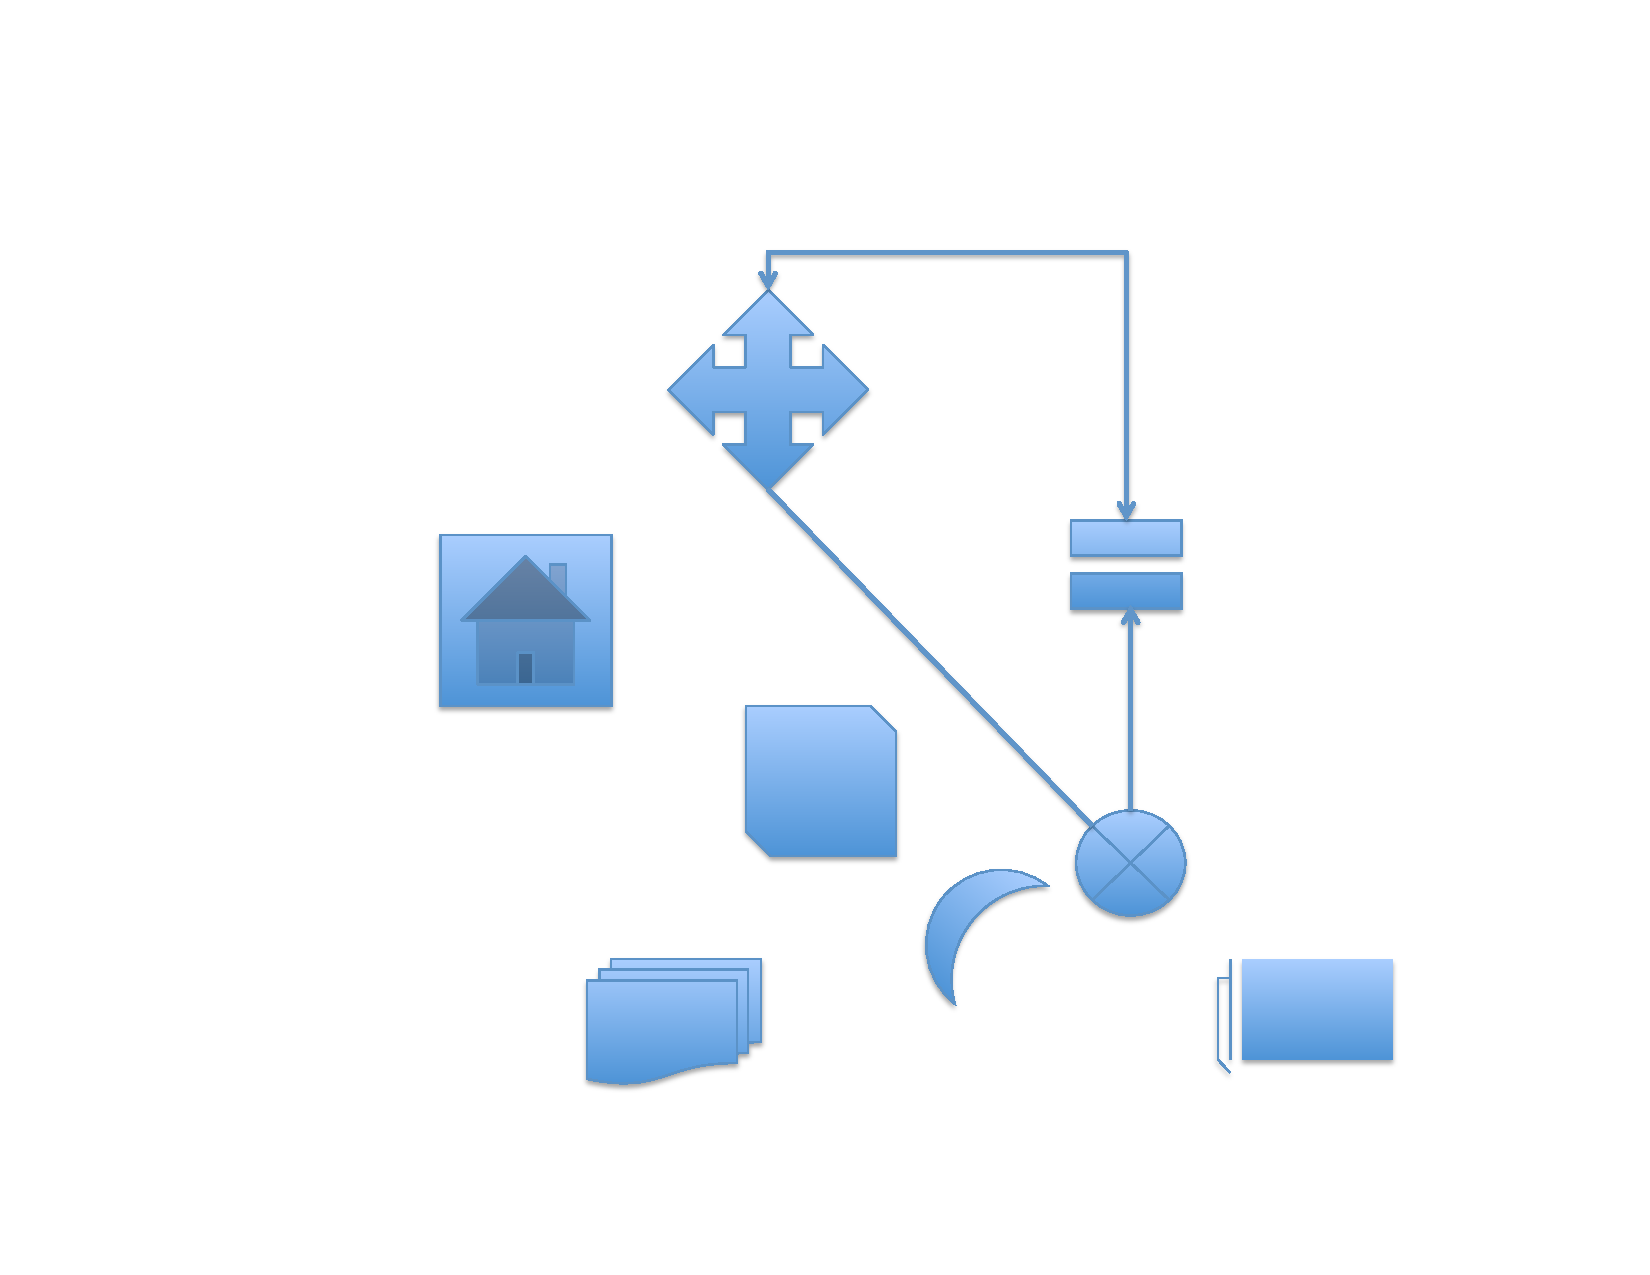
\includegraphics[width=6in]{./pics/my_figure}
\caption{Caption for my figure3}
\label{fig:MyFigure3}
\end{figure}



\begin{figure}
\centering 
	\begin{tikzpicture}[>=latex]
		% Draw the lines at multiples of pi/12
		\foreach \ang in {0,...,31} {
			\draw [lightgray] (0,0) -- (\ang * 180 / 16:4);
		}
		
		% Concentric circles and radius labels
		\foreach \s in {0, 1, 2, 3} {
			\draw [lightgray] (0,0) circle (\s + 0.5);
			\draw (0,0) circle (\s);
			\node [fill=white] at (\s, 0) [below] {\scriptsize $\s$};
		}
		
		% Add the labels at multiples of pi/4
		\foreach \ang/\lab/\dir in {
			0/0/right,
			1/{\pi/4}/{above right},
			2/{\pi/2}/above,
			3/{3\pi/4}/{above left},
			4/{\pi}/left,
			5/{5\pi/4}/{below left},
			7/{7\pi/4}/{below right},
			6/{3\pi/2}/below} {
			\draw (0,0) -- (\ang * 180 / 4:4.1);
			\node [fill=white] at (\ang * 180 / 4:4.2) [\dir] {\scriptsize $\lab$};
		}
		
		% The double-lined circle around the whole diagram
		\draw [style=double] (0,0) circle (4);
		
		\fill [fill=red!50!black, opacity=0.5] plot [domain=-pi/2:pi/2]
			(xy polar cs:angle=\x r, radius= {2-2*sin(\x r)});
		\draw [thick, color=red, domain=0:2*pi, samples=200, smooth]
			plot (xy polar cs:angle=\x r, radius={2-2*sin(\x r)});
		\node [fill=white] at (2,1) {$r=2-2\sin\theta$};
	\end{tikzpicture}
\caption{My polar plot}
\label{tikz:MyPolarPlot}
\end{figure}



\begin{figure}[h]
\centering 

\includegraphics[height=1.5in]{./pics/trim}
\caption{Caption for my figure4}
\label{fig:MyFigure4}
\end{figure}

















%%%%%%%%%%%%%%%%%%%%%%%%%%%%%%%%%%%%%%%%%
%	Typesetting Algorithms
%	This is written by Zhiyang Ong as a template for writing algorithms in LaTeX.

%	The MIT License (MIT)

%	Copyright (c) <2014> <Zhiyang Ong>

%	Permission is hereby granted, free of charge, to any person obtaining a copy of this software and associated documentation files (the "Software"), to deal in the Software without restriction, including without limitation the rights to use, copy, modify, merge, publish, distribute, sublicense, and/or sell copies of the Software, and to permit persons to whom the Software is furnished to do so, subject to the following conditions:

%	The above copyright notice and this permission notice shall be included in all copies or substantial portions of the Software.

%	THE SOFTWARE IS PROVIDED "AS IS", WITHOUT WARRANTY OF ANY KIND, EXPRESS OR IMPLIED, INCLUDING BUT NOT LIMITED TO THE WARRANTIES OF MERCHANTABILITY, FITNESS FOR A PARTICULAR PURPOSE AND NONINFRINGEMENT. IN NO EVENT SHALL THE AUTHORS OR COPYRIGHT HOLDERS BE LIABLE FOR ANY CLAIM, DAMAGES OR OTHER LIABILITY, WHETHER IN AN ACTION OF CONTRACT, TORT OR OTHERWISE, ARISING FROM, OUT OF OR IN CONNECTION WITH THE SOFTWARE OR THE USE OR OTHER DEALINGS IN THE SOFTWARE.

%	Email address: echo "cukj -wb- 23wU4X5M589 TROJANS cqkH wiuz2y 0f Mw Stanford" | awk '{ sub("23wU4X5M589","F.d_c_b. ") sub("Stanford","d0mA1n"); print $5, $2, $8; print " "; for (i=1; i<=1; i++) print "6\b"; print $9, $7, $6 }' | sed y/kqcbuHwM62z/gnotrzadqmC/ | tr 'q' ' ' | tr -d "\n" | tr -d 'ir' | tr y "\n"

%%%%%%%%%%%%%%%%%%%%%%%%%%%%%%%%%%%%%%%%%%%%%%



%%%%%%%%%%%%%%%%%%%%%%%%%%%%%%%%%%%%%%%%%%%
\chapter{Algorithms}
\label{chp:Algorithms}

A template for typesetting algorithms is shown in {\sc Procedure} \ref{lst:MyAlgorithm}.

\begin{codebox}
\Procname{$\proc{NAME OF THE ALGORITHM}({\it ARGUMENTS})$}
\label{lst:MyAlgorithm}
\zi \Comment {\it Input ARGUMENT \#1: Definition1}
\zi \Comment {\it Input ARGUMENT \#2: Definition2}
\li BODY OF THE PROCEDURE
\zi \Comment {\it A while loop.}
\li \While [condition]
	\Do
\li	[Something]
	\End
\zi \Comment {\it A for loop.}
\li \For \id{Var} $\gets$ [initial value] \To [final value]
	\Do
\li	[Something]
	\End
\zi \Comment {\it An if-elseif-else block.}
\li	\If $[$Condition1$]$
	\Then
\li		Blah\dots
\li	\ElseIf $[$Condition2$]$
	\Then
\li		Blah\dots
\li	\ElseIf $[$Condition3$]$
	\Then
\li		Blah\dots
%	\li	\ElseNoIf $[$Condition$]$
%		\Then
%	\li		Blah\dots
\li	\Else
\li		Blah\dots	
	\End
\zi \Comment {\it A variable assignment.}
\li $\id{blah} \gets A[j]$
\zi	\>	\Comment {\it This is indented with a tab.}
\zi	\Comment {\it What is the output of this procedure?}
\li	\Return
\end{codebox}







%%%%%%%%%%%%%%%%%%%%%%%%%%%%%%%%%%%%%%%%%
%	Bibliography
%\input{./others/bibliography}




%%%%%%%%%%%%%%%%%%%%%%%%%%%%%%%%%%%%%%%%%%%%%
%%%%%%%%%%%%%%%%%%%%%%%%%%%%%%%%%%%%%%%%%%%%%
%
%	End of document
%
%	Inserting references
%
%%%%%%%%%%%%%%%%%%%%%%%%%%%%%%%%%%%%%%%%%%%%%
%%%%%%%%%%%%%%%%%%%%%%%%%%%%%%%%%%%%%%%%%%%%%
%	Beginning of BACK MATTER: bibliography, indexes and colophon
%\backmatter
\appendix

{\linespread{1}
\bibliographystyle{plain}
\bibliography{./references/references}
\addcontentsline{toc}{chapter}{Bibliography}
}
\end{document}